This problem is solved using the set of point $S$ produced by the algorithm \ref{algStaticGuard}. Based on the knowledge of this points, clearing the whole area can be done easily. It is enough to have each guard visiting once each of this points to guarantee that there is no static intruder (since the whole area will be seen). Figure \ref{dynamicPath} shows the paths for 2 vehicles cleaning an area.

This problem and its solution are the following:

\begin{subproblem}
 Knowing the set of point $S$ and with a given number $n_{G}$ of guard, find the minimum path for each guard with the following condition:
 \begin{itemize}
  \item Each point has been seen once,
  \item The time to visit each point of $S$ is the smallest possible.
 \end{itemize}
This problem is quiet similar to the vehicles routing problem.
\label{subProb3}
\end{subproblem}

\begin{algorithm}
This algorithm gives a way to find the smallest path for a set of $n_{G}$ vehicle to visit a set $S = P_{1\leq i \leq n_S}$ of point.
\begin{enumerate}
  \item Create a matrix \textbf{Cost} with $\text{\textbf{Cost}}_{i,j} = \text{Length}(P_i,P_j)$ (real path length).
  \item Index each point of $S$ from $1$ to $n_{S}$.
  \item Index each guard from $n_{S}+1$ to $ n_{S}+n_{G}$. 
  \item Generate a valid permutation of $\{1,\hdots,n_{S}+n_{G}\}$ (see criteria \ref{permCriteria}).
  \item Compute the total length represented by the permutation using the matrix \textbf{Cost}.
  \item Keep this permutation in memory if its the best so far.
  \item While there is valid permutations go to 4.
\end{enumerate}
\label{dynamicGuard}
\end{algorithm}

\begin{figure}[h!t]
	\begin{center}
	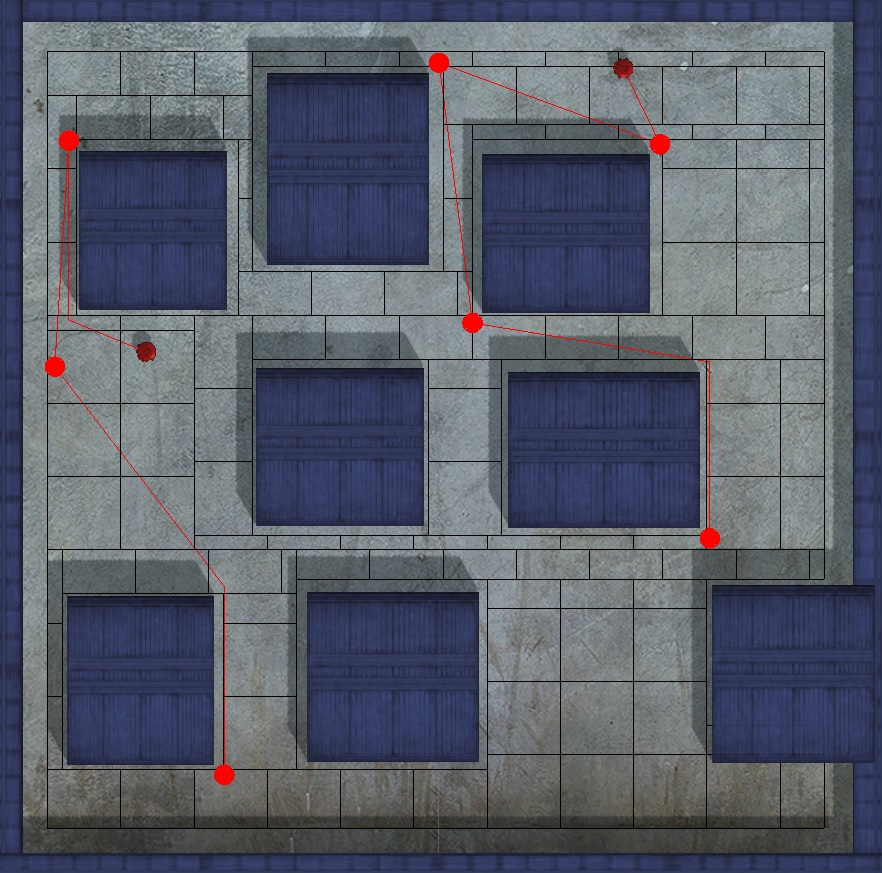
\includegraphics[width=\linewidth,natwidth=824,natheight=823]{fig/dynamicPath.jpg}
	\end{center}
	\caption{Path for $2$ vehicles looking for a static intruder}
	\label{dynamicPath}
\end{figure}

\subsection{Permutation}

Since there is $n!$ permutations for a set of $n$ elements, getting rid of a maximum of permutations is necesserary to achieve the algorithm in a decent time. 

\begin{criteria}
 The following criteria is used to know if a permutation based on the set $S$ and $n_G$ guards is valid or not:
 \begin{itemize}
  \item Each index in $\{1,\hdots,n_S\}$ has a predecessor stricly bigger than $n_S$ (it means that each point is visited once).
  \item Each indices in $\{n_S+1,\hdots,n_S+n_G\}$ are in ascending order.
  \item Each robot visit a maximum of $\left \lceil{\frac{n_P}{n_G}}\right \rceil$ (ceil function).
 \end{itemize}
 \label{permCriteria}
\end{criteria}